\begin{tikzpicture}[scale=.5]
\node (H1) at (225bp,-125bp)[draw,circle,fill=white] {$\mu_1$};
\node (H2) at (425bp,-125bp)[draw,circle,fill=white] {$\mu_2$};
\node (H3) at (425bp,-325bp)[draw,circle,fill=white] {$\mu_3$};
\node (H4) at (225bp,-325bp)[draw,circle,fill=white] {$\mu_4$};
\only<2,5,6,8>{\draw [line width=1pt] (H1) to (325bp, -124bp) node[fill=blue!20] {$H_{1}$} to (H2);}
\only<2,4,7,8>{\draw [line width=1pt] (H1) to (275bp, -175bp) node[fill=blue!20] {$H_{2}$} to (H3);}
\only<2,3,6,7,9>{\draw [line width=1pt] (H2) to (425bp, -224bp) node[fill=blue!20] {$H_{4}$} to (H3);}
\only<3,4,6,8,9,10>{\draw [line width=1pt] (H3) to (326bp, -324bp) node[fill=blue!20] {$H_{6}$} to (H4);}
\only<4,5,6,7>{\draw [line width=1pt] (H4) to (225bp, -227bp) node[fill=blue!20] {$H_{3}$} to (H1);}
\only<3,5,7,8,9,10>{\draw [line width=1pt] (H4) to (374bp, -176bp) node[fill=blue!20] {$H_{5}$} to (H2);}
\only<9,10>{\draw [line width=2pt,color=red,dashed] (H1) to (325bp, -124bp) node[fill=blue!20] {$H_{1}$} to (H2);}
\only<9,10>{\draw [line width=2pt,color=red,dashed] (H1) to (275bp, -175bp) node[fill=blue!20] {$H_{2}$} to (H3);}
\only<9>{\draw [line width=2pt,color=red,dashed] (H2) to (425bp, -224bp) node[fill=blue!20] {$H_{4}$} to (H3);}


\end{tikzpicture}
